\section{组合 PRG}

在本节中,我们将讨论两种构造,以允许我们基于旧的 PRG 建立新的 PRG。这些构造允许我们扩展原始 PRG 的输出空间的大小,同时保留其安全性。更重要的是,在本节中我们将介绍一种非常重要的论证技术,称为\textbf{混合论证 (hybrid argument)},该技术在现代密码学中的应用非常广泛。

\subsection{一种并行构造}\label{subsec:3-4-1}

令 $G$ 是一个定义在 $(\mathcal S,\mathcal R)$ 上的 PRG。假设在某些应用中,我们想多次使用 $G$。我们希望$G$的所有输出与$\mathcal{\rm R}$上的随机元素是计算上无法区分的。如果 $G$ 是一个安全的 PRG,并且种子是独立产生的,那么这样的$G$就能满足这个要求。

我们可以将 $G$ 的多个应用建模为一个新的 PRG $G'$。也就是说,我们构建一个新的PRG $G'$,它将$G$应用于$n$个种子,并将输出连接起来。因此,$G'$定义在 $(\mathcal S^n,\mathcal R^n)$ 上,对于 $s_1,\dots,d_n\in\mathcal S$,我们有:
$$
G'(s_1,\dots,s_n):=\big(G(s_1),\dots,G(s_n)\big)
$$
我们称 $G'$ 为 $G$ 的 \textbf{$n$ 次并行组合 ($n$-wise parallel composition)},$n$ 称为\textbf{重复参数 (repetition parameter)},并且,我们要求$n$是一个多项式边界的值。

\begin{theorem}\label{theo:3-2}
如果 $G$ 是一个安全的 PRG,那么 $G$ 的 $n$ 次并行组合 $G'$ 也是一个安全的 PRG。
\begin{quote}
特别地,对于每一个如攻击游戏 \ref{game:3-1} 中那样攻击 $G'$ 的 PRG 对手 $\mathcal A$,都存在一个如攻击游戏 \ref{game:3-1} 中那样攻击 $G$ 的 PRG 对手 $\mathcal B$,其中 $\mathcal B$ 是围绕 $\mathcal A$ 的一个基本包装器,满足:
\end{quote}
$$
{\rm PRG\mathsf{adv}}[\mathcal{A},G']=n\cdot{\rm PRG\mathsf{adv}}[\mathcal{B},G]
$$
\end{theorem}

作为热身,我们首先在 $n=2$ 的特殊情况下证明这个定理。令 $\mathcal A$ 是一个有效 PRG 对手,在攻击游戏 \ref{game:3-1} 中攻击 $G'$ 时有优势 $\epsilon$。我们想证明,如果 $G$ 是一个安全 PRG,则 $\epsilon$ 可以忽略不计。为此,我们把\textbf{游戏 $\mathbf{0}$} 定义为攻击游戏 \ref{game:3-1} 中的实验 $0$。这个游戏中的挑战者的工作方式如下:

\vspace*{5pt}

\hspace*{5pt} 计算 $s_1\overset{\rm R}\leftarrow\mathcal S$,$r_1\leftarrow G(s_1)$\\
\hspace*{26pt} 计算 $s_2\overset{\rm R}\leftarrow\mathcal S$,$r_2\leftarrow G(s_2)$\\
\hspace*{26pt} 将 $(r_1,r_2)$ 发送给 $\mathcal A$。

\vspace*{5pt}

\noindent
令 $p_0$ 为 $\mathcal A$ 在该游戏中输出 $1$ 的概率。

下面,我们定义\textbf{游戏$\mathbf{1}$},它在 $\mathcal A$ 和一个挑战者之间进行,其工作方式如下:

\vspace*{5pt}

\hspace*{2pt} \colorbox{gray!50}{计算 $r_1\overset{\rm R}\leftarrow\mathcal R$}\\
\hspace*{26pt} 计算 $s_2\overset{\rm R}\leftarrow\mathcal S$,$r_2\leftarrow G(s_2)$\\
\hspace*{26pt} 将 $(r_1,r_2)$ 发送给 $\mathcal A$。

\vspace*{5pt}

\noindent
请注意,游戏 $1$ 既不对应于攻击游戏 \ref{game:3-1} 中的实验 $0$,也不对应于实验 $1$;相反,它是一个``混合"实验,对应于实验$0$和实验$1$之间的某个状态。 我们所做的就是在游戏 $0$ 中用一个真随机值取代伪随机值 $r_1$(见上面的高亮行)。直观地说,在假设 $G$ 是一个安全 PRG 的情况下,对手 $\mathcal A$ 应该注意不到这种差异。为了更精确地论证这一点,令 $p_1$ 是 $\mathcal A$ 在游戏 $1$ 中输出 $1$ 的概率。

令 $\delta_1:=|p_1-p_0|$。我们声称,假设 $G$ 是一个安全的 PRG,则 $\delta_1$ 是可忽略不计的。事实上,我们很容易构建一个有效 PRG 对手 $\mathcal B_1$,他在攻击游戏 \ref{game:3-1} 中攻击 $G$ 的优势正好等于 $\delta_1$。对手 $\mathcal B_1$ 的工作方式如下:

\vspace*{5pt}

\hspace*{5pt} 当收到来自挑战者的 $r\in\mathcal R$,$\mathcal B_1$ 扮演 $\mathcal A$ 的挑战者的角色:\\
\hspace*{50pt} 令 $r_1\leftarrow r$\\
\hspace*{50pt} 计算 $s_2\overset{\rm R}\leftarrow\mathcal S$,$r_2\leftarrow G(s_2)$\\
\hspace*{50pt} 将 $(r_1,r_2)$ 发送给 $\mathcal A$。\\
\hspace*{26pt} 最后,$\mathcal B_1$ 输出 $\mathcal A$ 所输出的任何东西。

\vspace*{5pt}

\noindent
请注意,当 $\mathcal B_1$ 在其攻击游戏的实验 $0$ 中时,它完全模仿挑战者在游戏 $0$ 中的行为,而在实验 $1$ 中,它完全模仿挑战者在游戏 $1$ 中的行为。因此,$p_0$ 等于 $\mathcal B_1$ 在攻击游戏 \ref{game:3-1} 的实验 $0$ 中输出 $1$ 的概率,而 $p_1$ 等于 $\mathcal B_1$ 在攻击游戏 \ref{game:3-1} 的实验 $1$ 中输出 $1$ 的概率。因此,$\mathcal B_1$ 在攻击 $G$ 时的优势恰好是 $|p_1-p_0|$,正如我们上面声称的。

接下来,我们定义\textbf{游戏$\mathbf{2}$},它在 $\mathcal A$ 和一个挑战者之间进行,其工作方式如下:

\vspace*{5pt}

\hspace*{5pt} 计算 $r_1\overset{\rm R}\leftarrow\mathcal R$\\
\hspace*{23pt} \colorbox{gray!50}{计算 $r_2\overset{\rm R}\leftarrow\mathcal R$}\\
\hspace*{26pt} 将 $(r_1,r_2)$ 发送给 $\mathcal A$。

\vspace*{5pt}

\noindent
我们所做的就是把游戏 $1$ 中的伪随机值 $r_2$ 替换成一个真正的随机值(见上面的高亮行)。令 $p_2$ 为 $\mathcal A$ 在游戏 $2$ 中输出 $1$ 的概率。请注意,游戏 $2$ 对应于攻击游戏 \ref{game:3-1} 的实验 $1$,因此 $p_2$ 等于攻击游戏 \ref{game:3-1} 的实验 $1$ 中 $\mathcal A$ 相对于 PRG $G'$ 输出 $1$ 的概率。

令 $\delta_2:=|p_2-p_1|$。通过与上面类似的论证,很容易看到当 $G$ 是一个安全的 PRG 时,$\delta_2$ 是可忽略不计的。事实上,我们很容易构建一个有效 PRG 对手 $\mathcal B_2$,他在攻击游戏 \ref{game:3-1} 中攻击 $G$ 的优势正好等于 $\delta_2$。对手 $\mathcal B_2$ 的工作方式如下:

\vspace*{5pt}

\hspace*{5pt} 当收到来自挑战者的 $r\in\mathcal R$,$\mathcal B_2$ 扮演 $\mathcal A$ 的挑战者的角色:\\
\hspace*{50pt} 计算 $r_1\overset{\rm R}\leftarrow\mathcal R$\\
\hspace*{50pt} 令 $r_2\leftarrow r$\\
\hspace*{50pt} 将 $(r_1,r_2)$ 发送给 $\mathcal A$。\\
\hspace*{26pt} 最后,$\mathcal B_2$ 输出 $\mathcal A$ 所输出的任何东西。

\vspace*{5pt}

\noindent
$p_1$ 显然就等于 $\mathcal B_2$ 在攻击游戏 \ref{game:3-1} 的实验 $0$ 中输出 $1$ 的概率,而 $p_2$ 等于 $\mathcal B_2$ 在攻击游戏 \ref{game:3-1} 的实验 $1$ 中输出 $1$ 的概率。

回顾一下,我们有$\epsilon={\rm PRG\mathsf{adv}}[\mathcal{A},G']$,那么从上面的讨论中,我们有:
$$
\epsilon=|p_2-p_0|=|p_2-p_1+p_1-p_0|\leq|p_1-p_0|+|p_2-p_1|=\delta_1+\delta_2
$$
由于 $\delta_1$ 和 $\delta_2$ 都可忽略不计,那么$\epsilon$ 也可忽略不计(见事实 \ref{fact:2-6})。

这就完成了 $G'$ 在 $n=2$ 情况下的安全证明。在给出一般情况下的证明之前,我们先给出 $n=2$ 情况下的另一种证明方式。我们的第一个证明采用了构建两个对手 $\mathcal B_1$ 和 $\mathcal B_2$ 的方法,而第二个证明会把这两个对手合并为一个单一的如同攻击游戏 \ref{game:3-1} 中攻击 $G$ 的 PRG 对手 $\mathcal B$,其工作方式如下:

\vspace*{5pt}

\hspace*{5pt} 当收到来自挑战者的 $r\in\mathcal R$ 时,$\mathcal B$ 进行以下操作:\\
\hspace*{50pt} 随机选取 $\omega\in\{1,2\}$\\
\hspace*{50pt} 将 $r$ 发送给 $\mathcal B_\omega$。\\
\hspace*{26pt} 最后,$\mathcal B$ 输出 $\mathcal B_\omega$ 所输出的任何东西。

\vspace*{5pt}

记 $W_0$ 为 $\mathcal B$ 在攻击游戏 \ref{game:3-1} 的实验 $0$ 中输出 $1$ 的事件,$W_1$ 为 $\mathcal B$ 在攻击游戏 \ref{game:3-1} 的实验 $1$ 中输出 $1$ 的事件。以 $\omega=1$ 和 $\omega=2$ 为条件,我们有:
$$
\begin{aligned}
\Pr[W_0]
&=\Pr[W_0\,|\,\omega=1]\Pr[\omega=1]+\Pr[W_0\,|\,\omega=2]\Pr[\omega=2]\\
&=\frac{1}{2}\Big(\Pr[W_0\,|\,\omega=1]+\Pr[W_0\,|\,\omega=2]\Big)\\
&=\frac{1}{2}(p_0+p_1)
\end{aligned}
$$
类似地,我们也有:
$$
\begin{aligned}
\Pr[W_1]
&=\Pr[W_1\,|\,\omega=1]\Pr[\omega=1]+\Pr[W_1\,|\,\omega=2]\Pr[\omega=2]\\
&=\frac{1}{2}\Big(\Pr[W_1\,|\,\omega=1]+\Pr[W_1\,|\,\omega=2]\Big)\\
&=\frac{1}{2}(p_1+p_2)
\end{aligned}
$$
因此,如果 $\delta$ 是 $\mathcal B$ 在攻击游戏 \ref{game:3-1} 中相对于 $G$ 的优势,我们就有:
$$
\delta=\big\lvert\Pr[W_1]-\Pr[W_0]\big\rvert
=\bigg\lvert\frac{1}{2}(p_1+p_2)-\frac{1}{2}(p_0+p_1)\bigg\lvert
=\frac{1}{2}|p_2-p_0|
={\epsilon}/{2}
$$
即 $\epsilon=2\delta$。由于 $\delta$ 可忽略不计,$\epsilon$ 也可以忽略不计(见事实 \ref{fact:2-6})。

下面,我们正式介绍当 $n$ 为一个普通的,多项式边界的值时,定理 \ref{theo:3-2} 的证明。

\begin{proof}[证明思路]
我们可以尝试将上述第一种策略从 $n=2$ 的情况扩展到任意的 $n$ 的情况。也就是说,我们可以构建一个由 $n+1$ 个游戏构成的游戏序列。挑战者在开始时产生一个伪随机序列 $G(s_1),\dots,G(s_n)$,每次用 $\mathcal R$ 上的真随机元素替换其中的一个元素,最终得到一个 $\mathcal R$ 上的真随机序列 $(r_1,\dots,r_n)$。直觉上,对手应该注意不到这些替换中的哪怕任何一个,因为 $G$ 是一个安全的 PRG;然而,正式证明这一点需要构建 $n$ 个不同的对手,每个对手以稍微不同的方式去攻击 $G$。事实上,当 $n$ 不是一个绝对的常数,而单纯只是一个多项式边界的值时,这会导致一些恼人的技术困难;而扩展上面概述的第二种策略则要简单得多,因为这只需要构建一个对手,就能够``一击即中"地攻击 $G$。
\end{proof}

\begin{proof}
令 $\mathcal A$ 是一个有效 PRG 对手,他对 $G'$ 进行攻击游戏 \ref{game:3-1} 中的攻击。我们首先引入一个大小为 $n+1$ 的\textbf{混合游戏(hybrid games)}序列,称为混合$0$,混合$1$,$\dots$,混合$n$。对于$j=0,1,\dots,n$,混合 $j$ 是一个 $\mathcal A$ 和挑战者之间的游戏。挑战者会准备一个 $n$ 个值的元组,其中的前 $j$ 个元素是真随机值,其余的 $n-j$ 个元素是由 $G$ 输出的伪随机值;也就是说,挑战者的工作方式如下:

\vspace*{5pt}

\hspace*{5pt} $r_1\overset{\rm R}\leftarrow\mathcal R$\\
\hspace*{50pt} $\vdots$\\
\hspace*{26pt} $r_j\overset{\rm R}\leftarrow\mathcal R$\\
\hspace*{26pt} $s_{j+1}\overset{\rm R}\leftarrow\mathcal{S},\;r_{j+1}\leftarrow G(s_{j+1})$\\
\hspace*{50pt} $\vdots$\\
\hspace*{26pt} $s_{n}\overset{\rm R}\leftarrow\mathcal{S},\;r_{n}\leftarrow G(s_{j+1})$\\
\hspace*{26pt} 将 $(r_1,\dots,r_n)$ 发送给 $\mathcal A$。

\vspace*{5pt}

\noindent
像之前一样,$\mathcal A$ 在游戏结束时输出 $0$ 或 $1$。图 \ref{fig:3-5} 展示了挑战者在这 $n+1$ 个游戏中的每个游戏中准备的数值。令 $p_j$ 为 $\mathcal A$ 在混合 $j$ 中输出 $1$ 的概率。注意,$p_0$ 等于 $\mathcal A$ 在攻击游戏 \ref{game:3-1} 的实验 $0$ 中输出 $1$ 的概率,而 $p_n$ 则等于 $\mathcal A$ 在实验 $1$ 中输出 $1$ 的概率。因此,我们有:
\begin{equation}\label{eq:3-9}
{\rm PRG\mathsf{adv}}[\mathcal{A},G']=|p_n-p_0|
\end{equation}

\begin{figure}
  \centering
  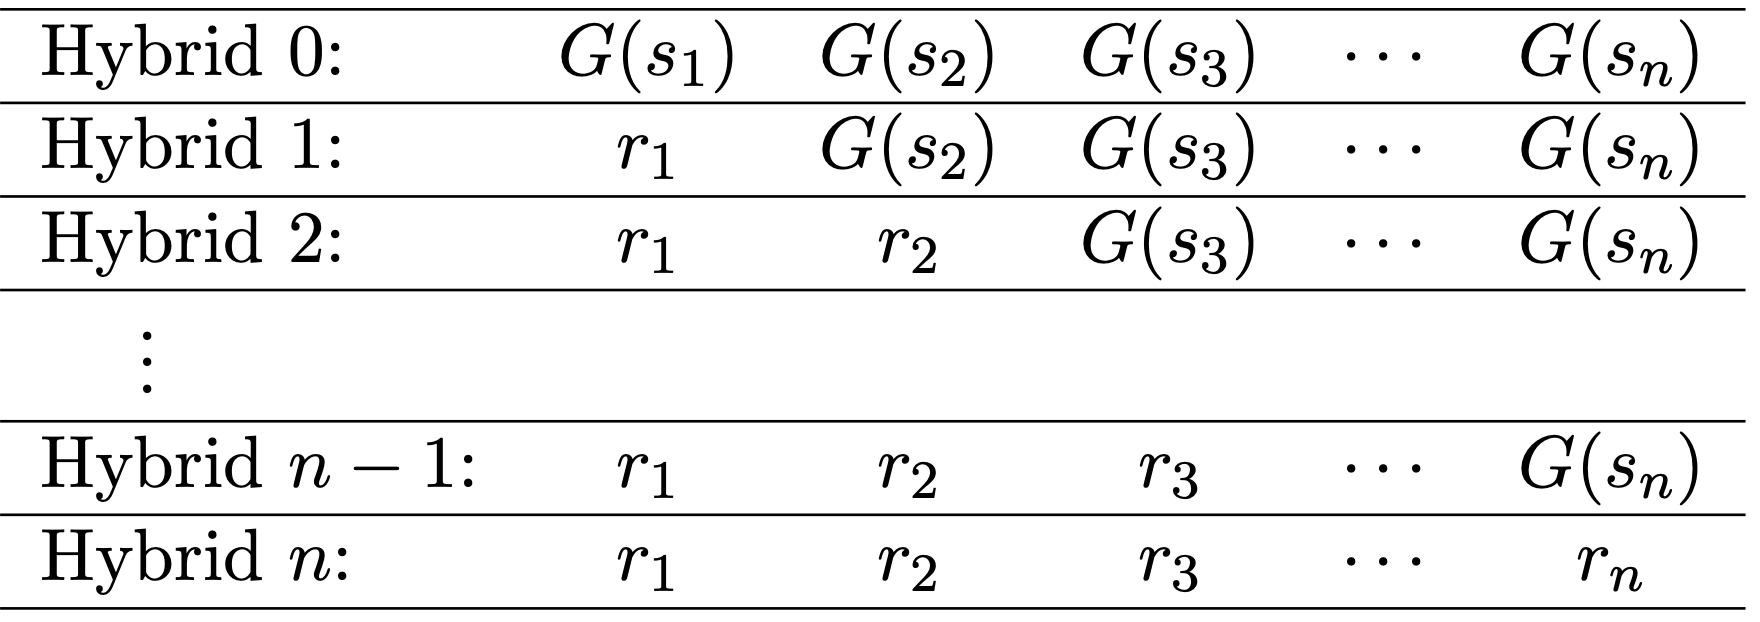
\includegraphics[width=0.55\linewidth]{figures/chapter3/fig5.png}
  \caption{挑战者在混合$0,1,\dots,n$中准备的数值。每个$r_i$都是$\mathcal{R}$上的一个随机元素,每个$s_i$都是$\mathcal{S}$上的一个随机元素。}
  \label{fig:3-5}
\end{figure}

接下来我们定义一个 PRG 对手 $\mathcal B$,它对 $G$ 进行攻击游戏 \ref{game:3-1} 中的攻击,其工作方式如下:

\vspace*{5pt}

\hspace*{5pt} 当收到来自挑战者的 $r\in\mathcal R$,$\mathcal B$ 扮演 $\mathcal A$ 的挑战者的角色:\\
\hspace*{50pt} $\omega\overset{\rm R}\leftarrow\{1,\dots,n\}$\\
\hspace*{50pt} $r_1\overset{\rm R}\leftarrow\mathcal R$\\
\hspace*{74pt} $\vdots$\\
\hspace*{50pt} $r_{\omega-1}\overset{\rm R}\leftarrow\mathcal R$\\
\hspace*{50pt} $r_{\omega}\leftarrow r$\\
\hspace*{50pt} $s_{\omega+1}\overset{\rm R}\leftarrow\mathcal{S},\;r_{\omega+1}\leftarrow G(s_{\omega+1})$\\
\hspace*{74pt} $\vdots$\\
\hspace*{50pt} $s_{n}\overset{\rm R}\leftarrow\mathcal{S},\;r_{n}\leftarrow G(s_{j+1})$\\
\hspace*{50pt} 将 $(r_1,\dots,r_n)$ 发送给 $\mathcal A$。\\
\hspace*{26pt} 最后,$\mathcal B$ 输出 $\mathcal A$ 所输出的任何东西。

\vspace*{5pt}

令 $W_0$ 是$\mathcal B$ 在攻击游戏 \ref{game:3-1} 的实验 $0$ 中输出 $1$ 的事件,$W_1$ 是$\mathcal B$在攻击游戏 \ref{game:3-1} 的实验 $1$ 中输出 $1$ 的事件。一个关键的观察是:

\begin{quote}
\emph{对于每个固定的 $j=1,\dots,n$,以 $\omega=j$ 为条件,$\mathcal B$ 的攻击游戏的实验 $0$ 就相当于混合 $j-1$,而 $\mathcal B$ 的攻击游戏的实验 $1$ 则相当于混合 $j$。
}
\end{quote}
因此:
$$
\Pr[W_0\,|\,\omega=j]=p_{j-1},\quad
\Pr[W_1\,|\,\omega=j]=p_{j}
$$
所以,我们有:
$$
\Pr[W_0]
=\sum_{j=1}^n\Pr[W_0\,|\,\omega=j]\Pr[\omega=j]
=\frac{1}{n}\sum_{j=1}^n\Pr[W_0\,|\,\omega=j]
=\frac{1}{n}\sum_{j=1}^np_{j-1}
$$
类似地:
$$
\Pr[W_1]
=\sum_{j=1}^n\Pr[W_1\,|\,\omega=j]\Pr[\omega=j]
=\frac{1}{n}\sum_{j=1}^n\Pr[W_1\,|\,\omega=j]
=\frac{1}{n}\sum_{j=1}^np_{j}
$$
最终,我们有:
$$
\begin{aligned}
{\rm PRG\mathsf{adv}}[\mathcal{B},G]
&=|\Pr[W_1]-\Pr[W_0]|\\
&=\Bigg\lvert\frac{1}{n}\sum_{j=1}^np_j-\frac{1}{n}\sum_{j=1}^np_{j-1}\Bigg\rvert\\
&=\frac{1}{n}|p_n-p_0|
\end{aligned}
$$
将其与式 \ref{eq:3-9} 相结合,我们可以得到:
$$
{\rm PRG\mathsf{adv}}[\mathcal{A},G']=n\cdot{\rm PRG\mathsf{adv}}[\mathcal{B},G]
$$
由于我们假设 $G$ 是一个安全 PRG,因此 ${\rm PRG\mathsf{adv}}[\mathcal{B},G]$ 可以忽略不计,而由于 $n$ 是多项式边界的,${\rm PRG\mathsf{adv}}[\mathcal{B},G']$ 也是可忽略不计的(见事实 \ref{fact:2-6})。这就证明了该定理。
\end{proof}

定理 3.2 表明,PRG 的安全性随着我们使用它的次数增多而最多呈线性下降。有人可能会问,这个约束是否是严格的?也即,安全性是否真的会随着使用次数的增加而线性下降?答案其实是肯定的(见练习 3.14)。

\subsection{一种串行构造:Blum-Micali 方法}\label{subsec:3-4-2}

我们下面介绍一种由 Blum 和 Micali 发明的串行构造,它使用一个只稍做延展的 PRG,建立一个可以伸展到任意长度的 PRG。

令 $G$ 是一个定义在 $(\mathcal{S},\mathcal{R}\times\mathcal{S})$ 上的 PRG,其中 $\mathcal S$ 和 $\mathcal R$ 是有限集。对于每个多项式边界的值 $n\geq 1$,我们可以构造一个定义在 $(\mathcal{S},\mathcal{R}^n\times\mathcal{S})$ 上的新的 PRG $G'$。对于 $s\in\mathcal{S}$,我们令:

\vspace*{5pt}

\hspace*{5pt} $G'(s):=$\\
\hspace*{50pt} $s_0\leftarrow s$\\
\hspace*{50pt} 对于 $i\leftarrow1$ 到 $n$:\\
\hspace*{75pt} $(r_i,s_i)\leftarrow G(s_{i-1})$\\
\hspace*{50pt} 输出$(r_1,\dots,r_n,s_n)$

\vspace*{5pt}

\noindent
我们称 $G'$ 为 $G$ 的 \textbf{$n$ 次串行组合 ($n$-wise sequential composition)}。图 \ref{fig:3-6} 是 $n=3$ 时$G'$ 的示意图。

\begin{figure}
  \centering
  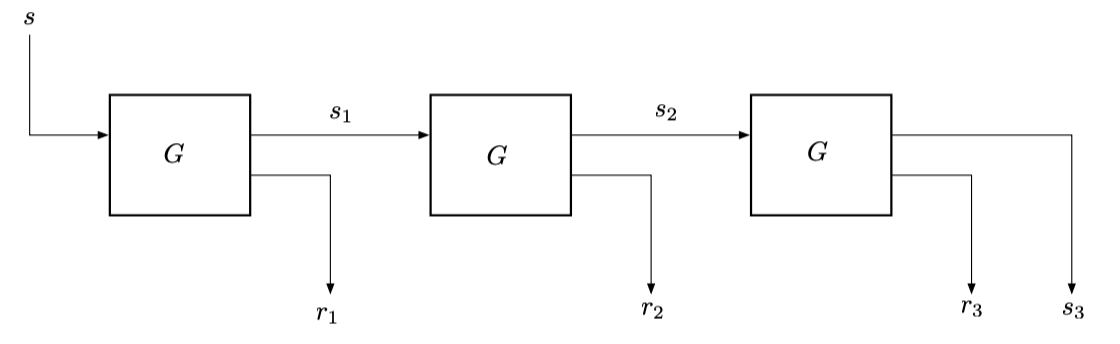
\includegraphics[width=0.8\linewidth]{figures/chapter3/fig6.png}
  \caption{$n=3$时的串行构造}
  \label{fig:3-6}
\end{figure}

我们将在下面的定理 \ref{theo:3-3} 中证明,如果 $G$ 是一个安全 PRG,那么 $G'$ 也是一个安全 PRG。作为这个构造的一个特例,假设 $G$ 是一个定义在 $(\{0,1\}^\ell,\{0,1\}^{t+\ell})$ 上的 PRG,其中 $\ell$ 和 $t$ 是正整数;也就是说,$G$ 把 $\ell$ 比特字符串拉伸为 $t+\ell$ 比特字符串。我们可以很自然地把 $G$ 的输出空间看作是 $\{0,1\}^t\times\{0,1\}^\ell$。应用上述构造,并把输出解释为比特串,我们就能得到一个PRG $G'$,它能把 $\ell$ 位比特串拉伸为 $nt+\ell$ 位比特串。

\begin{theorem}\label{theo:3-3}
如果 $G$ 是一个安全 PRG,那么 $G$ 的 $n$ 次串行组合 $G'$ 也是一个安全 PRG。
\begin{quote}
特别地,对于每个就 $G'$ 进行攻击游戏 \ref{game:3-1} 的 PRG 对手 $\mathcal A$,都存在一个就 $G$ 进行攻击游戏 \ref{game:3-1} 的 PRG 对手 $\mathcal B$,其中 $\mathcal B$ 是围绕 $\mathcal A$ 的一个基本包装器,满足:
\end{quote}
$$
{\rm PRG\mathsf{adv}}[\mathcal{A},G']=n\cdot{\rm PRG\mathsf{adv}}[\mathcal{B},G]
$$
\end{theorem}

\begin{proof}[证明思路]
该定理的证明是一个混合论证,其思路与定理 \ref{theo:3-2} 的证明非常相似。该证明背后的直觉如下所述。考虑一个 PRG 对手 $\mathcal A$,他在攻击游戏 \ref{game:3-1} 的实验 $0$ 中收到 $(r_1,\dots,r_n,s_n)$。由于 $s=s_0$ 是随机的,而且 $G$ 是一个安全 PRG,我们可以用 $\mathcal{R}\times\mathcal{S}$ 中的一个完全随机的元素来代替 $(r_1,s_1)$,且 $\mathcal A$ 在这个新的混合游戏中输出 $1$ 的概率应该只会发生可忽略不计的变化。现在,由于 $s_1$ 是随机的(同样是因为$G$ 是一个安全 PRG),我们就可以用 $\mathcal{R}\times\mathcal{S}$ 上的一个完全随机的元素来代替 $(r_2,s_2)$,而 $\mathcal A$ 在这第二个混合游戏中输出 $1$ 的概率应该也只会发生可忽略不计的变化。继续这样下去,我们可以用 $\mathcal{R}\times\mathcal{S}$ 中的随机元素逐步替换 $(r_3,s_3)$ 到 $(r_n,s_n)$,在做出这些改变之后,$\mathcal A$ 输出 $1$ 的概率应该都只会发生可忽略不计的变化(假设$n$是多项式边界的)。然而,在这一点上,$\mathcal A$ 输出 $1$ 的概率与他在攻击游戏 \ref{game:3-1} 的实验 $1$ 中输出 $1$ 的概率相同,因此,这个概率与$\mathcal A$在攻击游戏 \ref{game:3-1} 的实验 $0$ 中输出 $1$ 的概率接近得可以忽略不计。

这就是我们的想法;然而,就像在定理 \ref{theo:3-2} 的证明中一样,由于技术原因,我们设计了一个攻击$G$的 PRG 对手。
\end{proof}

\begin{proof}
令 $\mathcal A$ 是一个对 $G'$ 进行攻击游戏 \ref{game:3-1} 中的攻击的 PRG 对手。我们首先引入一个大小为 $n+1$ 的混合游戏序列,称为混合$0$,混合$1$,$\dots$,混合$n$。对于$j=0,1,\dots,n$,我们定义混合 $j$ 为 $\mathcal A$ 和以下挑战者之间的游戏。挑战者的工作方式如下:

\vspace*{5pt}

\hspace*{5pt} $r_1\overset{\rm R}\leftarrow\mathcal R$\\
\hspace*{50pt} $\vdots$\\
\hspace*{26pt} $r_j\overset{\rm R}\leftarrow\mathcal R$\\
\hspace*{26pt} $s_j\overset{\rm R}\leftarrow\mathcal S$\\
\hspace*{26pt} $(r_{j+1},s_{j+1})\leftarrow G(s_{j})$\\
\hspace*{50pt} $\vdots$\\
\hspace*{26pt} $(r_n,s_{n})\leftarrow G(s_{n-1})$\\
\hspace*{26pt} 将 $(r_1,\dots,r_n,s_n)$ 发送给 $\mathcal A$。

\vspace*{5pt}

\noindent
像之前一样,$\mathcal A$ 在游戏结束时输出 $0$ 或 $1$。图 \ref{fig:3-7} 展示了挑战者在 $n=3$ 的情况下的工作流程。请注意,$p_0$ 也等于 $\mathcal A$ 在攻击游戏 \ref{game:3-1} 的实验 $0$ 中输出 $1$ 的概率,而 $p_n$ 则等于 $\mathcal A$ 在攻击游戏 \ref{game:3-1} 的实验 $1$ 中输出 $1$ 的概率。因此,我们有:
\begin{equation}
{\rm PRG\mathsf{adv}}[\mathcal{A},G']=|p_n-p_0|
\end{equation}

接下来我们定义一个 PRG 对手 $\mathcal B$,它对 $G$ 进行攻击游戏 \ref{game:3-1} 中的攻击,其工作方式如下:

\vspace*{5pt}

\hspace*{5pt} 当收到来自挑战者的 $(r,s)\in\mathcal{R}\times\mathcal{S}$,$\mathcal B$ 扮演 $\mathcal A$ 的挑战者的角色:\\
\hspace*{50pt} $\omega\overset{\rm R}\leftarrow\{1,\dots,n\}$\\
\hspace*{50pt} $r_1\overset{\rm R}\leftarrow\mathcal R,\dots,r_{\omega-1}\overset{\rm R}\leftarrow\mathcal R$\\
\hspace*{50pt} $(r_{\omega},s_{\omega})\leftarrow(r,s)$\\
\hspace*{50pt} $(r_{\omega+1},s_{\omega+1})\leftarrow G(s_{\omega}),\dots,(r_n,s_n)\leftarrow G(s_{n-1})$\\
\hspace*{50pt} 将 $(r_1,\dots,r_n,s_n)$ 发送给 $\mathcal A$。\\
\hspace*{26pt} 最后,$\mathcal B$ 输出 $\mathcal A$ 所输出的任何东西。

\vspace*{5pt}

令 $W_0$ 是$\mathcal B$在攻击游戏 \ref{game:3-1} 的实验 $0$ 中输出 $1$ 的事件,$W_1$ 是$\mathcal B$在攻击游戏 \ref{game:3-1} 的实验 $1$ 中输出 $1$ 的事件。一个关键的观察是:
\begin{quote}
\emph{对于每个固定的 $j=1,\dots,n$,以 $\omega=j$ 为条件,$\mathcal B$ 的攻击游戏的实验 $0$ 等同于混合 $j-1$,而 $\mathcal B$ 的攻击游戏的实验 $1$ 则等同于混合 $j$。
}
\end{quote}
因此:
$$
\Pr[W_0\,|\,\omega=j]=p_{j-1},\quad
\Pr[W_1\,|\,\omega=j]=p_{j}
$$

\begin{figure}
  \centering
  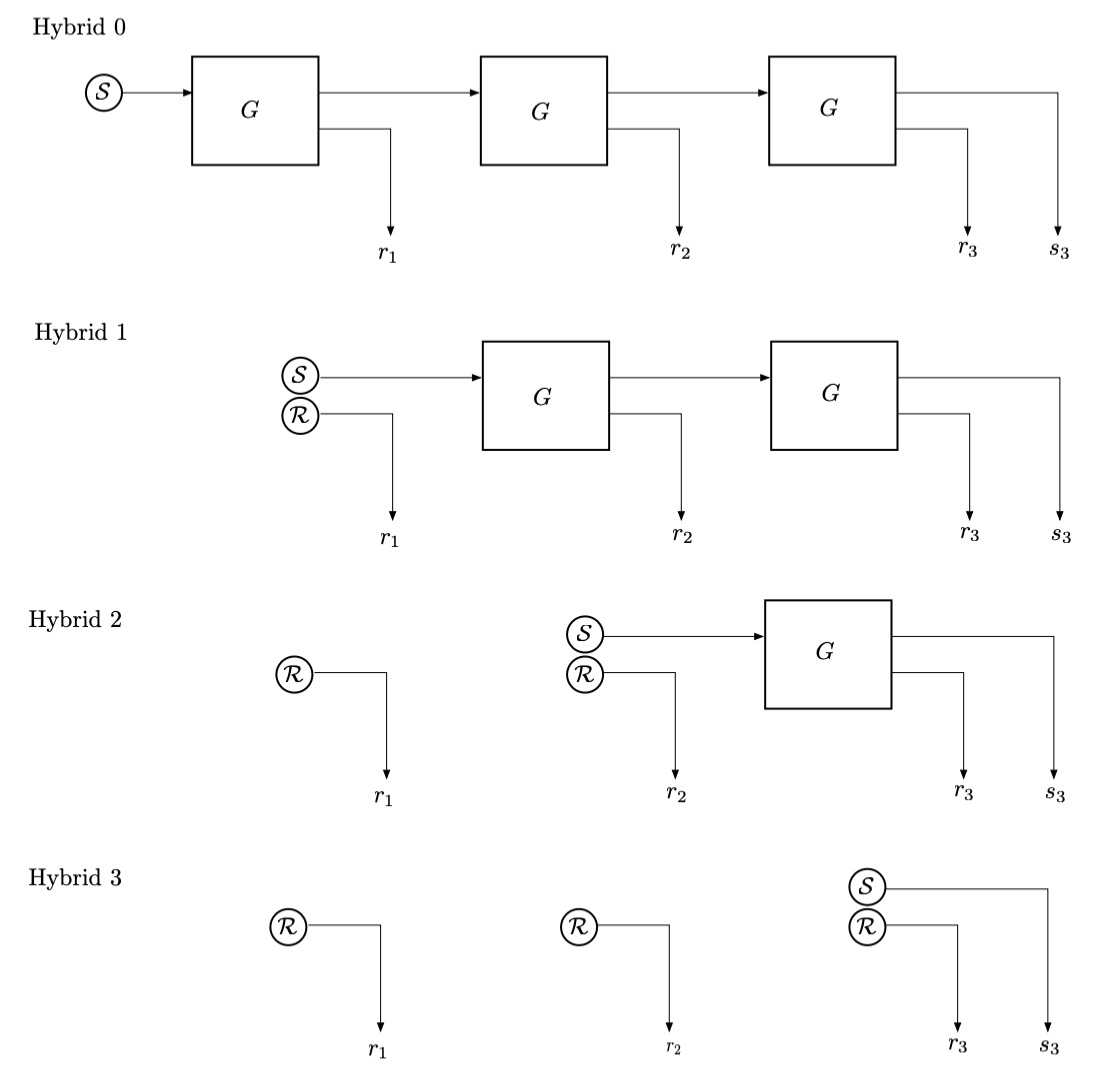
\includegraphics[width=0.8\linewidth]{figures/chapter3/fig7.png}
  \caption{$n=3$时,混合游戏中挑战者的计算。圆圈表示随机产生的$\mathcal{S}$或$\mathcal{R}$上的元素,如标签所示。}
  \label{fig:3-7}
\end{figure}

接下来的证明只是简单的计算,与定理 \ref{theo:3-2} 的证明的最后一段\emph{相同},不再赘述。
\end{proof}

评价 PRG 的一个标准是它的\textbf{扩展率 (expansion rate)}:一个将 $n$ 比特种子扩展到 $m$ 比特输出的 PRG 的扩展率为 ${m}/{n}$。更一般地说,如果种子空间是 $\mathcal{S}$,输出空间是 $\mathcal{\rm R}$,我们将扩展率定义为 ${\log|\mathcal{\rm R}|}/{\log|\mathcal{S}|}$。串行组合构造比并行组合构造提供了更好的扩展率,但是它有一个缺点,那就是它不能被并行化。事实上,存在一种构造可以兼顾两种优点:大的扩展率和高度可并行的结构,见 \ref{subsec:4-4-4} 小节。

\subsection{数学细节}

在定理 \ref{theo:3-2} 和 \ref{theo:3-3} 的证明中,有一些微妙的地方值得讨论。

首先,在这两个构造中,底层的 PRG $G$ 可能有系统参数。也就是说,可能存在一个概率性算法,它将安全参数 $\lambda$ 作为输入,并输出一个系统参数 $\Lambda$。回顾一下,系统参数是能够完全将构造实例化的公共数据(在这个场景中,它可能定义了种子空间和输出空间)。对于并行和串行构造,我们可以对 $G$ 的所有 $n$ 个实例使用相同的系统参数;事实上,对于串行构造来说,这是必须的,因为我们要确保一轮的输出可以被用作下一轮的输入。无论是对所有 $G$ 的实例使用相同的系统参数,还是对不同的实例使用不同的系统参数,这些安全定理的证明都是完全有效的。

其次,我们要简要讨论关于混合论证的一个相当深奥的问题。为了更具体一点,我们把注意力集中在定理 \ref{theo:3-2} 的证明上(尽管类似的讨论也适用于定理 \ref{theo:3-3} 的证明,或任何其他的混合论证)。在证明该定理时,我们最终想要证明,如果存在一个能破解 $G'$ 的有效对手 $\mathcal A$,那么也必然存在一个能破解 $G$ 的有效对手。假设 $\mathcal A$ 是一个能破解 $G'$ 的有效对手,那么它相对于 $G'$ 的优势 $\epsilon(\lambda)$(我们这里明确地把它表示成安全参数$\lambda$的一个函数)是不可忽略不计的。这意味着存在一个常数 $c$使得 $\epsilon(\lambda)\geq{1}/{\lambda^c}$适用于无限多的 $\lambda$。

现在,在定理 \ref{theo:3-2} 证明之前的讨论中,我们考虑了 $n=2$ 的特殊情况,并表明存在有效对手 $\mathcal{B}_1$ 和 $\mathcal{B}_2$,使得 $\epsilon(\lambda)\leq\delta_1(\lambda)+\delta_2(\lambda)$ 对于任意 $\lambda$ 都成立,其中 $\delta_j(\lambda)$ 表示 $\mathcal{B}_j$ 相对于 $G$ 的优势。由此可见,要么 $\delta_1(\lambda)\geq{1}/{2\lambda^c}$ 无限频繁,要么 $\delta_2(\lambda)\geq{1}/{2\lambda^c}$ 无限频繁。因此我们可以得出结论,要么是$\mathcal{B}_1$ 打破 $G$,要么是$\mathcal{B}_2$ 打破 $G$(也可能两者皆然)。因此,\emph{存在}一个能破解 $G$ 的有效对手:它要么是 $\mathcal{B}_1$ 要么是 $\mathcal{B}_2$,我们不知道到底是哪一个(也不必分清是哪一个)。然而无论是哪一个,它都是一个固定的对手,对所有的 $\lambda$ 都是统一定义的;也就是说,它是一个固定的,以 $\lambda$ 为输入的机器。

这个论证是完全有效的,并且可以扩展到任意\emph{常数} $n$:我们可以构造 $n$ 个对手 $\mathcal{B}_1,\dots,\mathcal{B}_n$,并论证对于某个 $j\in\{1,\dots,n\}$,对手 $\mathcal{B}_j$ 无限频繁地对 $G$ 有优势 ${1}/{n\lambda^c}$,从而攻破 $G$。然而这个论证并没有扩展到 $n$ 是 $\lambda$ 的函数的情况,我们现在把它明确写成 $n(\lambda)$。问题不在于 ${1}/({n(\lambda)\lambda^c})$ 也许太小(其实并不是)。这个问题相当微妙,所以在我们讨论它之前,让我们先回顾一下我们所给出的(合法)证明。对于每个 $\lambda$,我们定义一个大小为 $n(\lambda)+1$ 的混合游戏序列,因此对于每个 $\lambda$,我们实际上得到了一个不同的游戏序列。事实上,我们不能说有一个单一、有限的游戏序列对所有 $\lambda$ 都有效,因为 $n(\lambda)\to\infty$。尽管如此,我们还是明确地构造了一个固定的对手 $\mathcal B$,它是为所有 $\lambda$ 统一定义的;也就是说,$\mathcal B$ 是一个固定的机器,它把 $\lambda$ 作为输入。我们为每个 $\lambda$ 定义的混合游戏序列是一个数学对象,我们对其可计算性不做任何主张,它只是在分析 $\mathcal B$ 时使用的一个方便的工具。

希望到现在为止,读者至少对我们试图将常数 $n$ 的论证推广到一个函数 $n(\lambda)$ 时所产生的问题有了一个直观感觉。首先,我们甚至不清楚 $n(\lambda)$ 个对手 $\mathcal{B}_1,\dots,\mathcal{B}_{n(\lambda)}$ 是什么意思:我们的对手应该是将 $\lambda$ 作为输入的固定机器,而机器本身不应该依赖于 $\lambda$。撇开这种语言上的混乱不谈,我们对常数情况的证明只表明存在一个``对手",对于无限多的 $\lambda$ 值来说,它能以某种方式知道 $j=j(\lambda)$ 的``正确"值,以便在 $(n(\lambda)+1)$ 游戏混合论证中使用——没有一个 $j$ 常数值一定对无限多的 $\lambda$ 有效。如果使用非统一的计算模型,我们实际上可以使这种类型的论证有意义,但我们在本文中不会采取这种方法。

当我们使用一个构建单一对手 $\mathcal B$ 的混合论证时,所有这些问题都会消失,就像我们在定理 \ref{theo:3-2} 和 \ref{theo:3-3} 的证明中所做的。然而我们重申,我们在 $n=2$,或自然延伸到每一个常数 $n$ 的情况下所做的原始分析是完全有效的。在这种情况下,我们构建了一个单一、固定的 $n+1$ 游戏序列,每个单独的游戏对所有 $\lambda$ 都是统一定义的(就像我们的安全定义中的攻击游戏一样),我们还定义了一个有限的对手集合,每个对手都是一个固定的机器。我们重申这一点,因为在后面的内容中,我们将经常构建涉及这样的有限序列游戏的证明(事实上,定理\ref{theo:3-1}的证明就是这种类型)。在这种情况下,每个游戏将为所有 $\lambda$ 统一定义,并被称为游戏 $0$、游戏 $1$,等等。相反,当我们进行混合论证,使用非均匀的游戏序列时,我们将这些游戏表示为混合 $0$,混合 $1$ 等,以避免任何可能的混淆。